\documentclass{article}%
\usepackage[T1]{fontenc}%
\usepackage[utf8]{inputenc}%
\usepackage{lmodern}%
\usepackage{textcomp}%
\usepackage{lastpage}%
\usepackage{authblk}%
\usepackage{graphicx}%
%
\title{Ethanol Extracts of Fruiting Bodies of Antrodia cinnamomea Suppress CL1{-}5 Human Lung Adenocarcinoma Cells Migration by Inhibiting Matrix Metalloproteinase{-}2/9 through ERK, JNK, p38 and PI3K/Akt Signaling Pathways}%
\author{Emily Jones}%
\affil{National Creative Research Initiatives Center for Nuclear Receptor Signals, Hormone Research Center, School of Biological Sciences and Technology, Chonnam National University, Gwangju, Republic of Korea}%
\date{01{-}01{-}2013}%
%
\begin{document}%
\normalsize%
\maketitle%
\section{Abstract}%
\label{sec:Abstract}%
SAN DIEGO {-} A new treatment from the University of California, San Diego School of Medicine could treat the relapsing form of cerebral anemia that affects thousands of people in the United States and Europe.\newline%
In focal cerebral anemia {-}{-} the most common form of cerebral palsy and which affects about 50,000 people in the United States alone {-}{-} a condition in which the brain clears bleeding during healing or surgery, several arteries are injured and their flow can stop {-}{-} known as myocardial infarction.\newline%
Rituxan is one of the most commonly prescribed drugs for the condition. Rituxan also reduces blood pressure.\newline%
The new study, funded by the National Institutes of Health and published in Nature Medicine, is a work of immunology, research in which scientists use a naturally occurring protein, synapse{-}forming synapse, to stimulate the response of an immune system capable of removing foreign invaders in the body.\newline%
Copyright 2013 by Click2Houston.com. All rights reserved. This material may not be published, broadcast, rewritten or redistributed.

%
\subsection{Image Analysis}%
\label{subsec:ImageAnalysis}%


\begin{figure}[h!]%
\centering%
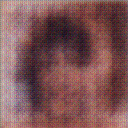
\includegraphics[width=150px]{500_fake_images/samples_5_191.png}%
\caption{A Close Up Of A Red And White Fire Hydrant}%
\end{figure}

%
\end{document}